\chapter{Grundlagen}
\label{ch:fundamentals}

Dieses Kapitel möchte einige Grundlagen definieren, welche im Kapitel~\ref{ch:main-matter} vorausgesetzt werden.
Es handelt von der Definition des funktionalen Programmier-Paradigma, welches in den Sprachen Clojure und Elm zum Einsatz kommt.
Weiterhin werden die Webtechnologien \acp{SPA} und Websockets erklärt, welche das Frontend des \nameref{ch:main-matter}'s nutzt. 
Die Architektur der ganzen Applikation wird maßgebend durch die Trennung in unabhängige Microservices beeinflusst, welche mit Docker realisiert sind.

\section{Eingesetzte Webtechnologien}
\subsection{\aclp{SPA}}
Einzelseiten-Webanwendungen (engl. \aclp{SPA}) stellen eine spezielle Art einer Webanwendung dar.
Sie unterscheiden sich zu einer klassischen Webseite dahingehend, dass sie nur aus einem einzelnen Html-Dokument bestehen und ihren Inhalt dynamisch nachladen.
Innerhalb dieser Einzelseite wird ebenso Java-Script-Code geladen, welcher die eigentliche Funktionalität enthält.
Oft weisen \acp{SPA} außerdem Merkmale von \acp{RIA} auf, da ihre Oberflächen typischerweise eher einer Desktop-Anwendung gleichen, als einer statischen Webseite. In diesem Kontext spricht man deswegen auch von so genannten Web-Apps.
\par
Da eine Verlagerung von sonst in einem Server enthaltene Präsentations-Logik stattfindet, resultiert diese Web-Architektur in einem Fat-Client.
Es wird dadurch die Serverlast reduziert und gleichzeitig die Grundlage für einen flüssigeren Übergang der Darstellung der Oberflächen geschaffen.
Alternativ dazu endet bei einer normalen Webseite der Präsentationsvorgang bei einem neuen Abfragen einer weiteren Unterseite.
\par
Um die zu nutzenden Daten zur Anzeige der Applikation zu erhalten, bedarf es einer gewissen Client-Architektur, welche einzelne \acs{AJAX}-Requests an eine (\acs{REST}-)Schnittstelle schickt, oder Nachrichten mit Hilfe einer beidseitigen Verbindung über Websockets sendet.
Seit in der Java-Script-Welt versucht wurde, das Konzept einer \ac{SPA} umzusetzen, war es schwierig, ein vernünftig wartbares System zu entwickeln.
Bekannte Vertreter von Libraries und Frameworks, welche die dabei anfallenden Probleme zu lösen versuchen, sind Google Angular und Angular 2, \ac{bzw.} Facebook React oder gänzlich neue Sprachen wie Elm oder Clojure-Script.

\subsection{Websockets}
Websocket-Verbindungen beruhen auf einem gleichnamigen Netzwerkprotokoll, welche eine beidseitige Client-Server-Kommunikation über \acs{TCP} ermöglichen.
Sie haben jedoch, wie ihr Name es vermuten lässt, wenig mit klassischen Unix-Sockets gemeinsam.
Entstanden sind sie aus dem Fehlen einer 

\section{Funktionale Programmierung}
Die funktionale Programmierung gehört zu den Deklarativen Programmierparadigmen und stellt neben der imperativen und objektorientierten Programmierung eines der am Häufigsten genutzten Paradigmen dar.
\par
Anders als bei imperativen Sprachen, unterscheiden sich funktionale Sprachen vor Allem an ihrer Unveränderbarkeit (engl. Immutability) von Variablen und ihrer Datenstrukturen.
Es wird dabei angestrebt, bei einer Veränderung des Zustandes (engl. State) einer Variablen nicht den Inhalt ihrer Referenz zu verändern, sondern stattdessen eine Kopie der Daten zurückzuliefern.
% In der Praxis hat sich vielfach herausgestellt, dass sich die häufig verwendete Veränderbarkeit (engl. Mutability) von Zuständen gerade auch in der objektorientierten Programmierung zu häufigen Fehlerquellen führen kann.
% Es wurde jedoch gezeigt, dass das Zurückgeben von Kopien ebenso sehr performant funktionieren kann {\bfseries (TODO: add quote)}.
\par
Wie der Name schon vermuten lässt basiert die funktionale Programmierung zu größten Teilen aus Funktionen. 
Diese sind meist als Module gekapselt, welche nach einer bestimmten Aufgabe gruppiert sind. 
Anders als bei Objekten möchte man offen mit den an die Funktionen übergebenen Daten umgehen und sie nicht in der Implementierung verstecken (engl. Information-Hiding). 
Dabei sollte eine Funktion nur diese eine Aufgabe erledigen, welche mithilfe ihres Namens beschrieben wird. 
Um dieses deterministische Verhalten zu erreichen, werden oft sehr granulare Funktionen erstellt, welche anschließend durch eine Komposition miteinander vereint werden\footnote{\texttt{f(x) = g(x) • h(x) <=> f(x) = h(g(x))}}.
Jegliche Seiteneffekte sollten vermieden werden, was man auch als reine (engl. pure) Funktionen bezeichnet.
So sollten Funktionen als Daten-Transformationen verstanden werden: Man erhält Daten, verarbeitet diese und gibt sie anschließend transformiert zurück, welches als \ac{EVA}-Prinzip bekannt ist.
\par
Da Funktionen selbst auch Typen darstellen, können sie ebenso als Parameter anderer Funktionen dienen, welche man dann auch als Funktionen Höherer Ordnung (engl. Higher Order Funktions) bezeichnet.
Mit dieser Voraussetzung können Verhalten aus einer aufzurufenden Funktion herausgelöst werden, womit das jeweilige Verhalten dynamisch bestimmt werden kann.
Diese Art von funktionen werden auch als Callbacks bezeichnet.
Hilfreich sind bei dieser Vorgehensweise auch so genannte Lamdas oder Closures, welche Funktionen darstellen, die inline definiert werden können und somit anonym \ac{bzw.} Unbenannt sind.
\par
Grundsätzlich werden funktionale Sprachen nochmals zwischen solchen Sprachen unterschieden, welche neben anderen Paradigmen auch das Funktionale Paradigma unterstützen und solchen, welche ausschließlich auf den Prinzipien der funktionalen Programmierung beruhen.
Die sogenannten reinen funktionalen Sprachen haben nicht einmal \ac{bspw.} die Möglichkeit Seiteneffekte auszuführen und sind sehr oft strikt typisiert.
In Multiparadigmensprachen beruhen viele funktionale Prinzipien und deren Erfolg, auf deren Einsatz und der generellen Bedachtheit des jeweiligen Programmierers \ac{bzw.} des einsetzenden Teams.
Man mag diese Prinzipien auch (Programming-)Patterns nennen, welche es zu befolgen, oder missverstehen gilt.

\section{Verwendete Programmiersprachen}
Das Projekt verwendet für den Server die Sprache Clojure, wohingegen der Client mithilfe von Elm umgesetzt ist.

\subsection{Clojure}
Die Sprache Clojure stellt einen modernen Lisp-Dialekt dar.
Sie ist eine Multiparadigmen-Sprache, möchte jedoch den Fokus auf funktionale Programmierung legen.
Ihre Quelldateien werden zu Java-Bytecode kompiliert und auf der Java-VM ausgeführt.
Clojure ist dynamisch typisiert, aber es existiert eine Bibliothek um Gradual-Typing zu ermöglichen.
Die bestehenden Datenstrukturen sind aufgrund ihrer Unveränderbarkeit (engl. Immutability) gerade auch für Einsatzzwecke geeignet, welche eine Nebenläufigkeit bzw. eine asynchrone Verarbeitung erfordern.
Durch die Interoperabilität zu Java kann auf deren umfassend bestehenden Bibliotheken innerhalb von Clojure-Code zugegriffen werden.
Ihre Bekanntheit hat Clojure \ac{u.A.} durch ihren speziellen Umgang von Zuständen erlangt ("`Separating Identity from State"').
\par
Ein weiteres bekanntes Merkmal ist das Konzept der Reducer (eager) bzw. Transducer (lazy).
Diese ermöglichen es, mehrere Transformationen an einer beliebigen Collection mit \ac{bspw.} \texttt{map, filter, reduce} zusammenzufassen (Komposition).
Dadurch kann die benötigte Zeit um die Transformationen auszuführen erheblich minimiert werden, weil nicht jede Teil-Transformation einzeln pro Element stattfindet, sondern gemeinsam.
Es existieren in einigen anderen Programmiersprachen\footnote{\ac{bspw.} in Elm: http://package.elm-lang.org/packages/avh4/elm-transducers/latest} Module, welche das Konzept der Transducer in ihrem Kontext umgesetzt haben.

\subsection{Elm}
Elm ist eine rein funktionale Programmiersprache, welche zu Java-Script kompiliert wird.
Die Syntax ist an ML-Artige Sprachen orientiert.
Sie wurde konzipiert um eine deklarativen Entwicklung von browserbasierten User-Interfaces zu ermöglichen.
Um Dinge wie HTML oder SVG abzubilden, existieren Funktionen, welche eine Liste an Eigenschaften eines Elements, sowie eine Liste seine Kinder erwarten.
Die Manipulationen an dem DOM des Browserfensters werden durch eine optimierte Vorgehensweise berechnet (Virtual DOM).
Ihr Compiler nutzt den statisch-typisierten Quellcode um eine möglichst hohe Developer-Experience (DX) zu gestalten.
So sind \ac{bspw.} seine Fehlermeldungen dazu gedacht, von Menschen gelesen zu werden.
Es ist eine Interoperabilität zu Java-Script über so genannte Ports möglich, welche die zugesicherte Typensicherheit gewährleistet.
Im Vergleich zu einfachem JS-Code, verspricht Elm keine Laufzeitfehler zu erzeugen, weil der Compiler durch das Typensystem sehr erfolgreich dabei ist Fehler zu finden.
\par
Es wird vorgeschlagen, seinen Code in Modulen zu kapseln, welche einer gewissen Struktur folgen, der sogenannten “`The-Elm-Architecture"' (TEA).
Diese setzt \ac{u.A.} das Vorhandensein jeweils einer \texttt{init-, update-} und \texttt{view-} Funktion und der Deklaration eines \texttt{Model}-Typs pro Modul voraus.
Eine \texttt{update-}Funktion verarbeitet Zustandsänderungen anhand dem Typen seiner eintreffenden \texttt{Message}.
Elm-\texttt{Messages} können \ac{bspw.} durch ein Klicken auf einen Button ausgelöst werden und können einen Payload enthalten.
Die einzelnen Typen von \texttt{Messages} können mithilfe eines Verbund-Datenyps (engl. Union-Type) beschrieben werden.
Es gibt einige Implementierungen von TEA in anderen Programmiersprachen.
Eines davon nennt sich \textit{Redux}, welches im Kontext von Java-Script View-Frameworks (\ac{bspw.} React) das State-Handling durch eine funktionale Herangehensweise strukturiert.
Eine ähnliche Architektur wurde von Facebook's Flux als "`One-Way Data-Flow"' vorgeschlagen.
\par
Weiterhin werden hilfreiche Abstraktionen wie von Websockets oder HTTP-Requests bereitgestellt, welche ebenso Elm-\texttt{Messages} auslösen.
In diesem Kontext sind auch die Elm-\texttt{Subscriptions} hilfreich, welche \ac{bspw.} ein kontinuierliches Reagieren auf Websocket-Ereignisse ermöglichen.

\section{Container-Virtualisierung mit Docker}
\begin{figure}
  \centering
  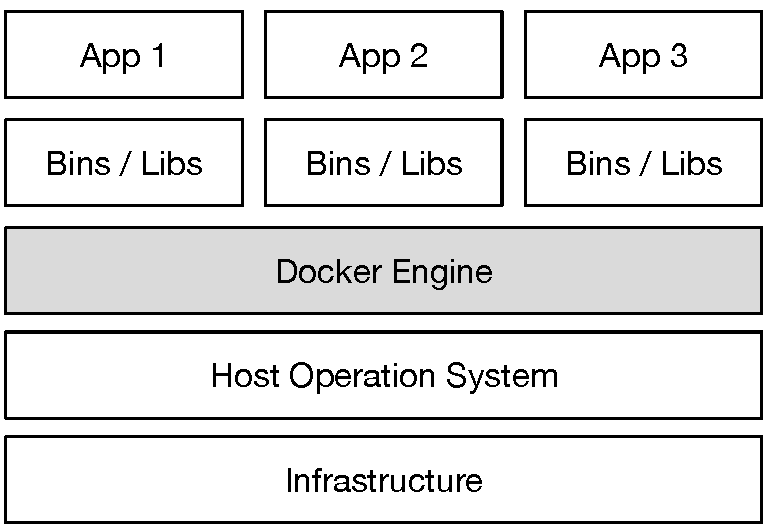
\includegraphics[scale=0.75]{docker.pdf}
  \par
  \caption{Schichten einer Virtualisierung mit Docker}
  \label{fig:layers-docker}
\end{figure}
Docker\footnote{\url{https://docs.docker.com/}} ist eine Software zum Deployment von Applikationen innerhalb von Containern.
Im Vergleich zu \acp{VM} ähnelt sich deren Vorgehensweise, jedoch laufen die Prozesse der Container direkt auf dem Host-Betriebssystem.
Grundlage dafür sind Bibliotheken, welche im Kernel oder sehr nah an diesem arbeiten, wohingegen klassische \acp{VM} durch ihre potenziell abstrakteren Zwischenschicht, weniger performant arbeiten können.
Trotz dieser Tatsache sind die Prozesse mithilfe von \ac{u.A.} Control-Groups und Kernel Namespaces voneinander isoliert.
Weiterhin hat man die Möglichkeit mit gängigen Mandatory-Access-Control-Frameworks wie SE-Linux oder App-Armor die Rechte innerhalb der Container zu beschränken.
Als Anforderung besteht keine spezifische Hardware-Infrastruktur wie bei beispielsweise VMWare ESXi.
Ebenso ist Docker mittlerweile auf allen gängigen Betriebssystemen lauffähig, wobei Linux-Derivate die beste Unterstützung erhalten.
Dies ist damit begründet, dass die Docker-Engine (\acs{Abb.}~\ref{fig:layers-docker}) auf den einzelnen Betriebssystemen verschieden aussieht.
\par
Ein Container wird mithilfe eines Dockerfiles beschrieben.
Darin werden deskriptive Instruktionen definiert um Abhängigkeiten zu installieren, Konfigurationen vorzunehmen und andere Build-Steps auszuführen.
Ein spezifischer Container wird als Image bezeichnet und setzt sich aus granularen Sub-Images zusammen.
Beim Erzeugen von Images eigener Dockerfiles müssen im Vergleich zu \acp{VM} keine großen Dateien transferiert werden, da sie aus ihrem Rezept reproduzierbar sind. 
Es besteht auch die Möglichkeit, von anderen Dockerfiles zu erben und diese über das Netzwerk verteilt bereitzustellen.
Falls die über eine Docker-Registry angebotenen Schichten eines Containers noch nicht auf dem eigenen Rechner vorhanden sind, so werden diese heruntergeladen.
\par
Weiterhin gibt es einen entscheidenden Vorteil gegenüber einer traditionellen \ac{VM}: Ein Dockerfile trägt implizit zur Dokumentation bei, da jede Änderung an einem Container in seinem Rezept ergänzt werden muss, um diese bei einem erneuten Start \ac{bzw.} erneuten Build zu erhalten.
\par
Wird eine Applikation in einzelnen Services aufgeteilt, so bietet sich das Tool \textbf{Docker-Compose}\footnote{\url{https://docs.docker.com/compose/overview/}} an.
Es ermöglicht in einer einzelnen Datei (\texttt{docker-compose.yml}) alle Konfigurations-Parameter der einzelnen Container zu definieren.
Das können \ac{bspw.} Volume-Mounts, Ports, Environment-Variables oder Netzwerke sein, welche sonst bei jedem \texttt{docker exec} Command angegeben werden müssten.
Alternativ dazu stünden eigene und oft fehlerintensive Shell-Scripts um ähnliches zu erreichen. 
\par
Es bietet sich auch an, getrennte Environments für Development, Test und Production als zentrale Dokumentation der Applikation zu nutzen (\texttt{docker-\break compose.[env].yml}).

